\chapter{Entropia di una o più variabili}

Nel precedente capitolo abbiamo introdotto il concetto di entropia di una sorgente, associandola al limite inferiore del costo di codifica per una sorgente binaria.
Tale trattazione è stata però piuttosto informale e non ha tenuto conto di alcune importanti proprietà dell'entropia.

In questo capitolo approfondiremo il concetto di entropia introdotto nel capitolo precedente, analizzandolo più formalmente, introducendo alcune sue proprietà e generalizzandolo a più variabili aleatorie.

\section{Rimandi di teoria della probabilità}

Prima di procedere, facciamo un breve richiamo ad alcuni concetti di teoria della probabilità necessari per la comprensione dei concetti che andremo a trattare in questo capitolo.
Un \keyword{spazio di probabilità} è una tripla \((\Omega, \mathcal{F}, \Prob)\) dove
\begin{itemize}
  \item \(\Omega\) è un insieme non vuoto, detto spazio campione;
  \item \(\mathcal{F} \subseteq \mathcal{P}(\Omega)\) è una \(\sigma\)-algebra su \(\Omega\), cioè un insieme di sottoinsiemi di \(\Omega\) che contiene \(\Omega\) stesso, è chiuso rispetto al complemento e alle unioni numerabili;
  \item \(\Prob: \mathcal{F} \to [0,1]\) è una misura di probabilità, cioè una funzione tale che \(\Prob[\Omega] = 1, \Prob[\emptyset] = 0\) e che è \(\sigma\)-additiva, ovvero per ogni famiglia numerabile di eventi disgiunti \(\{A_i\}_{i \in \mathbb{N}} \subseteq \mathcal{F}\) si ha che
  \[\Prob\left[\bigcup_{i=1}^{\infty} A_i\right] = \sum_{i=1}^{\infty} \Prob[A_i]\]
\end{itemize}

Una \keyword{variabile aleatoria discreta} su uno spazio di probabilità \((\Omega, \mathcal{F}, \Prob)\) è un applicazione misurabile \(S: \Omega \to \SCal\), dove \(\SCal\) è un insieme discreto (finito o numerabile).

Essendo \(S\) misurabile, è possibile associare una funzione \q{massa} di probabilità (distribuzione su \(\SCal\)) \(p: \SCal \to [0,1]\) definita come \(p(s) = \Prob[S=s] = \Prob[S^{-1}(s)]\)
Per allinearci alla notazione usata in teoria della probabilità, indicheremo con \(X,Y,Z\) le variabili aleatorie su \(\mathcal{X}, \mathcal{Y}, \mathcal{Z}\).

\begin{definition}{Entropia di una variabile aleatoria}
  Sia \(X\) variabile aleatoria discreta con distribuzione di probabilità \(p\).
  L'\keyword{entropia} di \(X\) è definita come
  \[H(X) = -\sum_{x \in \mathcal{X}} p(x) \log( p(x))\]
\end{definition}

A seguito del teorema di Shannon, possiamo interpretare questa quantità come il limite inferiore del costo di codifica per una sorgente binaria.
Dunque possiamo vedere l'entropia come la più corta descrizione binaria del valore di \(X\), o in altre parole il numero medio di domande binarie necessarie per identificare il valore di \(X\).

\begin{definition}{Definizione assiomatica dell'entropia di Shannon}
  Sia \({(H_m)}_{m \geq 1}\) una famiglia di funzioni, di cui ogni \(H_m \in {(H_m)}_{m \geq 1}\) è una funzione a \(m\) variabili con le seguenti proprietà:
  \begin{description}
    \item[simmetria]: \(\forall \sigma \in S_m, H_m(p_1,\ldots,p_m) = H_m(p_{\sigma(1)},\ldots,p_{\sigma(m)})\), con \( S_m\) insieme delle permutazioni di \(\set{1,\ldots,m}\).
    \item[normalizzazione]: \(H_2\left(\frac{1}{2}, \frac{1}{2}\right) = 1\).
    \item[continuità]: \(H_2(p,1-p)\) funzione continua di \(p\)
    \item[raggruppamento]:
    \[H_m(p_1,p_2,p_3,\ldots,p_m) = H_{m-1}(p_1 + p_2,p_3,\ldots,p_m)+(p_1+p_2)H_2(\frac{p_1}{p_1+p_2},\frac{p_2}{p_1+p_2})\]
  \end{description}
\end{definition}

Presa questa definizione, si ha necessariamente che \( H_m(p_1,\ldots,p_m) = - \sum_{i=1}^{m} p_i \log(p_i)\), preso un qualsiasi \(m\geq 1\).

Andiamo quindi a introdurre più variabili aleatorie, e a definire come si comporta l'entropia in questo caso.

\begin{definition}{Entropia Congiunta}
  Siano \(X, Y\) variabili aleatorie. Definiamo la \keyword{variabile aleatoria congiunta}, rappresentata dalla coppia \((X,Y)\), come:
  \[(X,Y): \omega \in \Omega \mapsto (X(\omega), Y(\omega)) \in \mathcal{X} \times \mathcal{Y}\]
  
  La cui funzione di massa di probabilità congiunta è data da
  \[p(x,y) = \Prob[X=x, Y=y] = \Prob[X=x \land Y=y] = \Prob[X^{-1}(x) \cap Y^{-1}(y)]\]
  L'\keyword{entropia congiunta} di \(X\) e \(Y\) è definita come
  \[H(X,Y) = - \sum_{\substack{x \in \mathcal{X},\\ y \in \mathcal{Y}}} p(x,y) \log(p(x,y)) = \EV{\log\left(\frac{1}{p(x,y)}\right)}\]
\end{definition}

\begin{definition}{Condizionamento}
  Dati \(A,B \subseteq \Omega\), definiamo \(A|B\) l'evento \(A\) condizionato a \(B\) come l'evento tale che
  \[\Prob[A|B] = \frac{\Prob[A \cap B]}{\Prob[B]}\]

  In particolare, se \(X,Y\) sono variabili aleatorie, definiamo \(p(y|x) = \Prob(Y=y|X=x)\)

  Si ha dunque che \(\forall x \in \mathcal{X}, y \in \mathcal{Y}, p(y|x) = \frac{p(x,y)}{p(x)}\), cioè \(p(x,y) = p(x)p(y|x)\).
\end{definition}

Possiamo notare che  \(\forall x \in \mathcal{X}\) fissato, \(p(y|x)\) è una distribuzione di probabilità su \(\mathcal{Y}\).
Infatti,\footnote{Si ricorda che, date \(X,Y\) variabili aleatorie, si ha che \(\sum_{y \in \mathcal{Y}} p(x,y) = p(x), \forall x \in \mathcal{X}\) per definizione di probabilità marginale.
Di conseguenza, data una probabiltà congiunta \(p(x,y)\), è sempre possibile ricavare le distribuzioni marginali di \(X\) e \(Y\), ma non il contrario.}
\[\sum_{y \in \mathcal{Y}} p(y|x) = \sum_{y \in \mathcal{Y}} \frac{p(x,y)}{p(x)} = \frac{1}{p(x)} \sum_{y \in \mathcal{Y}} p(x,y) = \frac{p(x)}{p(x)} = 1\]


Essendo dunque questa una distribuzione di probabilità, possiamo vederla come funzione massa di probabilità di una variabile aleatoria \(Y|X=x\).

\begin{definition}{Entropia Condizionata}
  Siano \(X,Y\) variabili aleatorie.
  L'\keyword{entropia condizionata} di \(Y|X\) è definita come
  \[H(Y|X) = \sum_{x \in \mathcal{X}} p(x) H(Y|X=x) = - \sum_{x \in \mathcal{X}} p(x) \sum_{y \in \mathcal{Y}} p(y|x) \log(p(y|x)) = \]
  \[= -\sum_{\substack{x \in \mathcal{X}\\y \in \mathcal{Y}}} p(x,y) \log (p(y|x)) = \EV{\log\left(\frac{1}{p(y|x)}\right)}[x,y]\]
  
  Ovvero la media delle entropie di \(Y|X=x\) al variare di \(x\), pesata secondo la probabilità \(p(x)\).
\end{definition}

Definite queste quantità, vediamo come si relazionano tra di loro, partendo dalla prima regola di catena.

\begin{proposition}{Regola di catena}
  Date \(X,Y\) variabili aleatorie, si ha che
  \[H(X,Y) = H(X) + H(Y|X)\]
\end{proposition}

\begin{proof}
  \todo{Aggiustare i passaggi}
  \[H(X,Y) =-\sum_{\substack{x \in \mathcal{X},\\ y \in \mathcal{Y}}} p(x,y) \log(p(x,y)) = -\sum_{\substack{x \in \mathcal{X},\\ y \in \mathcal{Y}}} p(x,y) \log(p(x)p(y|x)) = \]
  \[= - \sum_{\substack{x \in \mathcal{X},\\ y \in \mathcal{Y}}} p(x,y)\left(\log(p(x)) + \log(p(y|x))\right)  = - \sum_{\substack{x \in \mathcal{X},\\ y \in \mathcal{Y}}} p(x,y) \log(p(x)) - \sum_{\substack{x \in \mathcal{X},\\ y \in \mathcal{Y}}} p(x,y) \log(p(y|x)) =\]
  \[=- \sum_{x \in \mathcal{X}} \log(p(x))\sum_{y \in \mathcal{Y}} p(x,y)  - \sum_{\substack{x \in \mathcal{X},\\ y \in \mathcal{Y}}} p(x,y) \log(p(y|x)) = H(X) + H(Y|X)\]
\end{proof}

\begin{example}{}
  Prendiamo in considerazione due variabili aleatorie quaternarie \(X,Y\) la cui probabilità congiunta è data dalla seguente tabella:
  \begin{center}
    \begin{tabular}{c|c c c c}
      \(Y \backslash X\) & \(a\) & \(b\) & \(c\) & \(d\) \\
      \hline
      \(1\) & \(\frac{1}{8}\) & \(\frac{1}{16}\) & \(\frac{1}{32}\) & \(\frac{1}{32}\) \\
      \(2\) & \(\frac{1}{16}\) & \(\frac{1}{8}\) & \(\frac{1}{32}\) & \(\frac{1}{32}\) \\
      \(3\) & \(\frac{1}{16}\) & \(\frac{1}{16}\) & \(\frac{1}{16}\) & \(\frac{1}{16}\) \\
      \(4\) & \(\frac{1}{4}\) & \(0\) & \(0\) & \(0\) \\
    \end{tabular}
  \end{center}

  Verifichiamo che \(H(X) = \frac{7}{4}\).
  Per calcolare l'entropia di \(X\), dobbiamo prima calcolare la distribuzione di probabilità marginale di \(X\):
  \begin{itemize}
    \item \(p(a) = \frac{1}{8} + \frac{1}{16} + \frac{1}{16} + \frac{1}{4} = \frac{1}{2}\)
    \item \(p(b) = \frac{1}{16} + \frac{1}{8} + \frac{1}{16} + 0 = \frac{1}{4}\)
    \item \(p(c) = \frac{1}{32} + \frac{1}{32} + \frac{1}{16} + 0 = \frac{1}{8}\)
    \item \(p(d) = \frac{1}{32} + \frac{1}{32} + \frac{1}{16} + 0 = \frac{1}{8}\)
  \end{itemize}
  Abbiamo dunque che
  \[H(X) = \frac{1}{2}\log(2)+\frac{1}{4}\log(4)+\frac{1}{8}\log(8)+\frac{1}{8}\log(8) = \]
  \[= \frac{1}{2}+\frac{1}{4}\cdot 2 + \frac{2}{8} \cdot 3 = \frac{7}{4}\]
  
  Verifichiamo ora che \(H(Y) = 2\).
  Analogamente a prima, calcoliamo la distribuzione di probabilità marginale di \(Y\):
  \begin{itemize}
    \item \(p(1) = \frac{1}{8} + \frac{1}{16} + \frac{1}{32} + \frac{1}{32} = \frac{1}{4}\)
    \item \(p(2) = \frac{1}{16} + \frac{1}{8} + \frac{1}{32} + \frac{1}{32} = \frac{1}{4}\)
    \item \(p(3) = \frac{1}{16} + \frac{1}{16} + \frac{1}{16} + \frac{1}{16} = \frac{1}{4}\)
    \item \(p(4) = \frac{1}{4} + 0 + 0 + 0 = \frac{1}{4}\)
  \end{itemize}
  Dunque
  \[H(Y) = 4 \cdot \frac{1}{4} \log(4) = 2\]

  Verifichiamo ora che \(H(X,Y) = \frac{27}{8}\).
  In questo caso è sufficiente calcolare direttamente l'entropia congiunta:
  \[H(X,Y) = 2\cdot\frac{1}{8}\cdot 3 + 6\cdot\frac{1}{16}\cdot 4 + \frac{1}{4}\cdot 2 + 4 \cdot \frac{1}{32}\cdot 5= \]
  \[= \frac{6}{8} + \frac{24}{16} + \frac{2}{4} + \frac{20}{32} = \frac{27}{8}\]
  

  Infine, si ha che \(H(X|Y) = H(X,Y)-H(X) = \frac{27}{8} - \frac{7}{4} = \frac{13}{8}\) e che \(H(Y|X) = H(X,Y)-H(Y) = \frac{27}{8} - 2 = \frac{11}{8}\).
\end{example}

Da questi calcoli possiamo osservare come l'entropia congiunta sia simmetrica rispetto alle variabili coinvolte, mentre l'entropia condizionata no.
In generale quindi \(H(X|Y) \neq H(Y|X)\) e \(H(X,Y) = H(Y,X)\).


Dunque dalla regola di catena si ha che
\[H(Y)+H(X|Y)=H(Y,X)=H(X,Y) = H(X)+H(Y|X)\]
Ovvero
\[H(Y) - H(Y|X) = H(X) - H(X|Y)\]

Possiamo dunque andare a generallizare questi risultati a più variabili aleatorie.

\begin{proposition}{Regola di catena con condizionamento}
  Date \(X,Y,Z\) variabili aleatorie, si ha che
  \[H(X,Y|Z) = H(X|Z) + H(Y|X,Z)\]
  ossia
  \[- \sum_{\substack{x \in \mathcal{X},\\y\in\mathcal{Y},\\z \in \mathcal{Z}}} p(x,y,z) \log(p(x,y|z)) = -\sum_{\substack{x\in\mathcal{X},\\z\in\mathcal{Z}}} p(x,z)\log(p(x|z)) - \sum_{\substack{x \in \mathcal{X},\\y \in \mathcal{Y},\\z \in \mathcal{Z}}} p(x,y,z) \log(p(y|x,z))\]
\end{proposition}


\begin{definition}{Divergenza di Kullback-Leibler (entropia relativa)}
  Siano \(p,q\) due distribuzioni di probabilità su uno stesso insieme discreto \(\mathcal{X}\).
  La \keyword{divergenza di Kullback-Leibler} tra \(p\) e \(q\) è definita come
  \[D_{KL}(p ||q) = \sum_{x \in \mathcal{X}} p(x) \log\left(\frac{p(x)}{q(x)}\right) \]
\end{definition}

\begin{note}{}
  Essendo che possono esistere \(x\) tali che \(q(x) = 0\) e \(p(x) > 0\), la divergenza di Kullback-Leibler può essere infinita.
\end{note}

La divergenza di Kullback-Leibler è spesso interpretata come una distanza, anche se non ne rispetta propriamente le proprietà matematiche.

Infatti non sono soddisfatte la simmetria, \(D(p||q) \neq D(q||p)\), e la disuguaglianza triangolare.
La divergenza di Kullback-Leibler è però \textit{definita positiva}, ovvero \(D_{KL}(p||q) \geq 0\) con uguaglianza se e solo se \(p=q\).\footnote{Questo segue in maniera diretta dall'\Cref{eq:gibbs} vista in precedenza}

\begin{definition}{Mutua Informazione}
  Siano \(X,Y\) variabili aleatorie congiunte.
  La \keyword{mutua informazione} tra \(X\) e \(Y\) è definita come
  \[I(X;Y) = D_{KL}(p(x,y) || p(x)p(y)) = \sum_{\substack{x \in \mathcal{X}\\y \in \mathcal{Y}}} p(x,y) \log\left(\frac{p(x,y)}{p(x)p(y)}\right)\]

  Essendo che \(p(x,y)=p(x)p(y), \forall x\in\mathcal{X}, y\in\mathcal{Y} \iff\) \(X\) e \(Y\) sono indipendenti, si ha che \(I(X;Y) = 0 \iff\) \(X\) e \(Y\) sono indipendenti.
\end{definition}

Intuitivamente, la mutua informazione misura la quantità di informazione, come riduzione di incertezza, che una variabile aleatoria fornisce sull'altra.
Questa è ovviamente nulla quando le due variabili sono indipendenti.

Si ha inoltre che
\[I(X;Y) = \sum_{\substack{x \in \mathcal{X}\\y \in \mathcal{Y}}} p(x,y) \log\left(\frac{p(x,y)}{p(x)p(y)}\right) = \]
\[= \sum_{\substack{x \in \mathcal{X}\\y \in \mathcal{Y}}} p(x,y) \log\left(\frac{p(y|x)}{p(y)}\right) = \sum_{\substack{x\in\mathcal{X}\\y\in\mathcal{Y}}}p(x,y)\log(p(y|x)) - \sum_{y\in\mathcal{Y}}\log(p(y))\sum_{x\in\mathcal{X}}p(x,y)\]
\[= H(Y)-H(Y|X)\]


Un modo intuitivo per visualizzare le relazioni tra le varie quantità di informazione viste finora è tramite i diagrammi di Venn modificati come in \Cref{fig:venn_info}.

\begin{figure}[H]
  \centering
  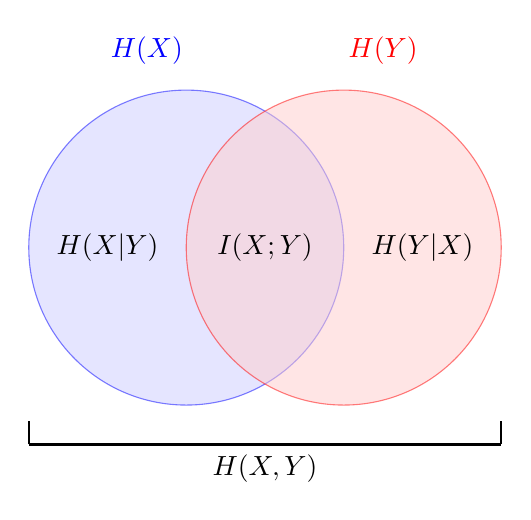
\begin{tikzpicture}
    \def \r {2} % radius of circles
    \def \d {2} % distance between centers

    % Draw circles
    \draw[fill=blue!20, draw=blue, opacity=0.5] (-\d/2,0) circle (\r);
    \draw[fill=red!20, draw=red, opacity=0.5] (\d/2,0) circle (\r);

    % Labels
    \node at (-\d/2-0.5, \r + 0.5) [blue] {\(H(X)\)};
    \node at (\d/2+0.5, \r + 0.5) [red] {\(H(Y)\)};
    \node at (0,0) {\(I(X;Y)\)};
    \node at (-\d, 0) {\(H(X|Y)\)};
    \node at (\d, 0) {\(H(Y|X)\)};

    \draw[thick] (-\d/2-\r,-\r-0.5) to node[midway, below, ] {\(H(X,Y)\)} (\d/2+\r,-\r-0.5);
    \draw[thick] (-\d/2-\r,-\r-0.5) -- ++(0,0.3);
    \draw[thick] (\d/2+\r,-\r-0.5) -- ++(0,0.3);
  \end{tikzpicture}
  \caption{Diagramma di Venn per le quantità di informazione}\label{fig:venn_info}
\end{figure}

\begin{definition}{Informazione mutua condizionata}
  Date \(X,Y,Z\) variabili aleatorie, la \keyword{mutua informazione condizionata} tra \(X\) e \(Y\) dato \(Z\) è definita come
  \[I(X;Y|Z) = H(X|Z) - H(X|Y,Z)\]
\end{definition}

Possiamo dunque generalizzare le regole di catena a \(n\) variabili.

\begin{proposition}{}
  Siano \(X_1, X_2, \ldots, X_n, Y\) variabili aleatorie.
  Si ha che
  \[H(X_1, X_2, \ldots, X_n) = H(X_1) + H(X_2|X_1) + \cdots + H(X_n | X_1, X_2, \ldots, X_{n-1}) = \]
  \[=H(X_1) + \sum_{i=2}^{n} H(X_i | X_{i-1}, \ldots, X_1)\]
  E che
  \[I(X_1, \ldots, X_n; Y) = I(X_1; Y) + I(X_2; Y | X_1) + \cdots + I(X_n; Y | X_1, \ldots, X_{n-1}) = \]
  \[=I(X_1;Y) + \sum_{i=2}^{n} I(X_i; Y | X_{i-1}, \ldots, X_1)\]
\end{proposition}

Andiamo dunque a definire gli estremi della mutua informazione.

Essendo \(I\) definita in termini di divergenza di Kullback-Leibler è definita positiva, dunque \(I(X;Y) \geq 0\) con uguaglianza se e solo se \(X\) e \(Y\) sono indipendenti.
In tal caso infatti, le due variabili non forniscono alcuna informazione l'una sull'altra.

Da un punto di vista formale, questo si ha perché \(p(x,y)=p(x)p(y)\) per ogni \(x \in \mathcal{X}\) e \(y \in \mathcal{Y}\) se e solo se \(X\) e \(Y\) sono indipendenti.

Per quanto riguarda l'estremo superiore, si ha che, essendo \(I(X;Y) = H(X) - H(X|Y)\), ed essendo \(H(X), H(X|Y) \geq 0\), \(I(X,Y)\) sarà massima quando \(H(X|Y) = 0\), ovvero quando \(X\) è funzione di \(Y\), ovvero\footnote{Ricordiamo che dati due insiemi \(A,B\), con \(B^A\) si intende l'insieme delle funzioni da \(A\) a \(B\), come visto nel primo capitolo.}
\[\exists f \in \mathcal{X}^\mathcal{Y} \st X= f\circ Y\]
Infatti, 
\[H(X|Y) = -\sum_{\substack{x\in\mathcal{X}\\y\in\mathcal{Y}}}p(x,y)\log(p(x|y)) = 0 \iff \forall x \in \mathcal{X}, y \in \mathcal{Y}, p(x,y)=0\lor p(x|y)=1\]
Essendo che fissato \(y\in\mathcal{Y}\), \(p(x|y)\) è una distribuzione di probabilità su \(\mathcal{X}\), si ha che
\[\forall y \in \mathcal{Y}, \exists! x:=f(y)\st p(x|y)=1\]